%!TEX root = ../../Main.tex
\graphicspath{{Chapters/Project/}}
%-------------------------------------------------------------------------------

\section{Convolutional Network architecture} % (fold)
\label{sec:convolutional_network_architecture}

A convolutional neural network consists of a number of different layers each transforming an 3D input volume of activations to an 3D output volume through a differentiable function. The different layers used in the networks of this project are described in this section. 

\subsection{Convolutional layers} % (fold)
\label{sub:conv_layers}

Convolutional layers are the core layers of a convolutional network. Regular
neural networks scales improperly to an increasing input space because each
neuron in one layer connects to all neurons in previous layers. The rationale behind introducing convolutional layers is to utilize the intrinsic spatially local correlation in natural images. This drastically reduces the amount of parameters in the network yet retaining great performance.

Convolutonal layers output a 3D volume (width x height x depth) comprised of neurons and the input is also a 3D volume, e.g. (32 x 32 x 3) as in CIFAR10 images. The neurons in the output volume are connected only to a local region in the input volume. This connectivity is determined by the receptive field of a neuron. The receptive field $F$ is a hyperparameter that describes the size of a filter that is being slided along the spatial dimension the input volume during forward pass. For every filter movement the dot product between the filter entries and input are calculated thus producing a activation map. The output volume consists of stacked activation maps along the depth dimension. The intuition of how the convolutional layer works is that the filters are learnable parameter that will activate on specific type of features in a region of the inputs spatial dimension.

In addition to the receptive field $F$ three other hyperparameters exists in a convolutional layer. These are the number of filters $K$, the stride $S$ and the amount of zero padding $P$ and together they control the size of the output volume. 

The depth $K$ regulate the number of neurons in the output volume that connects to the same spatial region of the input. Each neuron in the depth column will be trained to activate for distinct features. The number of learnable filters essentially determine the value of $K$.

The stride determines the spatial stepsize movement of the filter. If the
receptive field is $F = 7$ and the stride is $S = 1$ this would result in
neurons with considerable amount of overlapping of receptive fields and thus a
big number of depth columns. When the stride increases the receptive field
overlapping per neuron decrease which entails fewer depth columns in the output
volume.

Zero padding is the third hyperparameter $P$ that is concerned with the size of
the output volume. It describes the amount of zero padding, i.e. the number of
``zero layers'' put around the border of the input. Zero padding is useful if
preservation of the spatial dimensions of the input is desired.

As a rule of thumb it is recommended to use small filters ($F=3 \vee F=5$), a
small stride ($S=1 \vee S=2$) and with necessary padding in order to preserve
the input dimension \cite{cs231n}. Larger filter sizes are not unusual but these
are most often seen in convolutional layers close to the input image. A stride
$S=1$ is recommended as the convolutional layer then only will influence the
depth of a volume. A special pooling layer is dedicated to reduce the amount of
depth columns. This process is also known as downsampling. Pooling layers are
given special attention later in this report.

\subsection{ReLU layers} % (fold)
\label{sub:relu_layers}

Activation maps are often followed by an element-wise activation function. The Rectified Linear Unit (ReLU) is one of many activation function to choose among and are of special interest in this project. The ReLU activation function is the most common activation function in the lower layers of convolutional neural netorks. Other activation functions could be the Sigmoid or the Tanh activation functions.

The ReLU differs from the other mentioned activations function in several ways.
First of all it converges faster which results in shorter training time.
Secondly, the ReLU activation function do not saturate which avoids the problem
about the gradient getting killed which would lead to the case where the network
stops learning during training \cite{cs231n}. This problem is known from the use
of the other activation functions.

The formula for the ReLU activation function is very simple but efficient and
are as follows: $f(x)=max(0,x)$ and is illustrated in the figure \ref{fig:relu}.

\begin{figure}
  \centering
  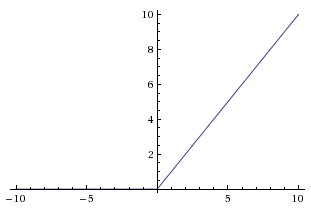
\includegraphics[scale=0.5]{Img/relu.jpeg}
  \caption{Illustration of the ReLU activation function}
  \label{fig:relu}
\end{figure}

% subsection conv_layers (end)

\subsection{Pooling layers} % (fold)
\label{sub:pool_layers}

Pooling layers are common in-between successive convolutional layers. The primary purpose of introducing pooling layers is to reduce the spatial dimensions of a volume hence alleviating computations needed when training the network. This essentially means that the number of parameters in the network decreases. Thus pooling layers also contribute to control overfitting.

Parameter reduction is achieved by performing downsampling. This is done by applying filters along the spatial dimension of a volume effectively discarding many of the activations. The filter size, or spatial extend $F$, and stride $S$ are hyperparameters that has to be chosen at time the model is being constructed. As stated in \cite{cs231n} most commonly seen pooling layers are either non-overlapping with $F=2, S=2$ or overlapping with $F=3, S=2$.

Various downsampling strategies exists. The ones that are of interest in this project are max and average pooling. Historically average pooling has been used however recently max pooling has shown to perform better in practice. To understand the intuition of this one might consider this rough analogy: Say a city has four districts and you know whether or not it rains in each district. You are then asked if it rains in the city. You would most likely look at each district and say yes if it is raining in any of the districts. This process resembles max pooling. You would probably not count the raining cities and divide by 4 as average pooling proposes. 

We can transfer this analogy to our ConvNet. If a feature is detected in a small region it is less likely to appear multiple times, unless the image is kind of blurry or ghosty. Calculating the mean of this region would result in a value that is lower than the actual value. In that sense average pooling is not ideal.

% subsection pool_layers (end)
\subsection{Fully-Connected Layers} % (fold)
\label{sub:fc_layers}

Having several convolutional layers, ReLU layers and pooling layers at some
point it is time for the high-level reasoning. A fully connected layer consist of neurons each being connected to all activations in the previous volume. Fully connected layers will transform the features into a space that is easier to classify. i.e. compute the class scores.

This project is restricted to the softmax classifier only, however different classifiers exists among these the popular Support Vector Machines (SVM).

The Softmax classifier gets its name from the softmax function which squeeze the raw class scores into values from 0 to 1 which sums to 1. This allows the cross-entropy loss to be applied. The cross-entropy loss takes the form:

$$ L_i = -log\left(\frac{e^{f_{y_i}}}{\sum_{j}{e^{f_j}}}\right)$$

When a convolutional network is said to be trained a loss function is essentially being minimized. This function/objective is comprised of two parts namely the data loss and regularization loss. The data loss part is the mean of $L_i$ over all training examples. The regularization loss part is present in order to prevent overfitting. Further explanation of regularization is considered out of scope of this project.

% subsection fc_layers (end)

% section convolutional_network_architecture (end)
